\documentclass{article}
\usepackage[T1]{fontenc}
\usepackage[paperwidth=6.6in,paperheight=1.72in,margin=0pt]{geometry}
\pagestyle{empty}
\usepackage{tikz}
\usetikzlibrary{arrows.meta, positioning, fit, backgrounds, calc}

\definecolor{warmBg}{HTML}{FFF3E0}
\definecolor{warmBorder}{HTML}{E0A050}
\definecolor{warmTitle}{HTML}{BF6A00}
\definecolor{coolBg}{HTML}{E3F2FD}
\definecolor{coolBorder}{HTML}{5090D0}
\definecolor{coolTitle}{HTML}{1565C0}
\definecolor{arrowColor}{HTML}{616161}
\definecolor{labelColor}{HTML}{424242}

\setlength{\topskip}{0pt}
\setlength{\parindent}{0pt}

\begin{document}
\vspace*{-3pt}%
\noindent
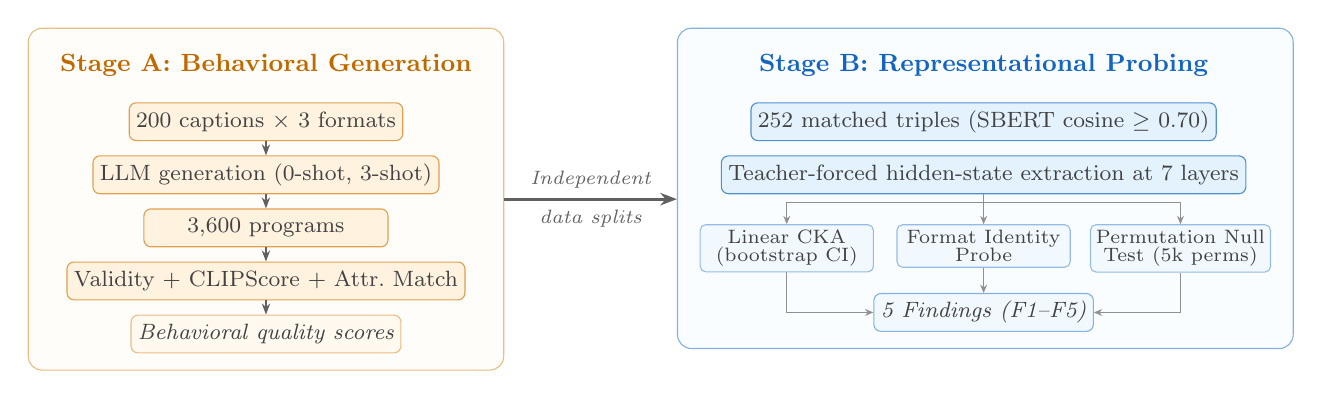
\begin{tikzpicture}[
    >=Stealth,
    font=\small,
    warmbox/.style={
        draw=warmBorder, fill=warmBg, rounded corners=2.5pt,
        minimum width=3.1cm, minimum height=0.48cm,
        align=center, inner sep=2.5pt, text=labelColor,
        font=\footnotesize
    },
    coolbox/.style={
        draw=coolBorder, fill=coolBg, rounded corners=2.5pt,
        minimum width=3.5cm, minimum height=0.48cm,
        align=center, inner sep=2.5pt, text=labelColor,
        font=\footnotesize
    },
    analysisbox/.style={
        draw=coolBorder!60, fill=coolBg!50, rounded corners=2pt,
        minimum width=2.2cm, minimum height=0.44cm,
        align=center, inner sep=2pt, text=labelColor,
        font=\scriptsize
    },
    resultbox/.style={
        rounded corners=2.5pt,
        minimum width=2.6cm, minimum height=0.48cm,
        align=center, inner sep=2.5pt, text=labelColor,
        font=\footnotesize\itshape
    },
    stagelabel/.style={font=\small\bfseries},
    midarrow/.style={
        -{Stealth[length=4pt,width=3pt]},
        arrowColor, line width=0.5pt
    },
    thinarrow/.style={
        -{Stealth[length=3pt,width=2.5pt]},
        arrowColor!70, line width=0.4pt
    },
]

% ============================================================
%  STAGE A
% ============================================================
\node[stagelabel, text=warmTitle] (stageA) {Stage A: Behavioral Generation};

\node[warmbox, below=0.2cm of stageA] (inputA)
    {200 captions $\times$ 3 formats};

\node[warmbox, below=0.18cm of inputA] (processA)
    {LLM generation (0-shot, 3-shot)};

\node[warmbox, below=0.18cm of processA] (outputA)
    {3{,}600 programs};

\node[warmbox, below=0.18cm of outputA, minimum width=3.3cm] (evalA)
    {Validity + CLIPScore + Attr.\ Match};

\node[resultbox, draw=warmBorder!70, fill=warmBg!50,
      below=0.18cm of evalA] (resultA)
    {Behavioral quality scores};

\draw[midarrow] (inputA) -- (processA);
\draw[midarrow] (processA) -- (outputA);
\draw[midarrow] (outputA) -- (evalA);
\draw[midarrow] (evalA) -- (resultA);

% ============================================================
%  STAGE B
% ============================================================
\node[stagelabel, text=coolTitle, right=3.4cm of stageA] (stageB)
    {Stage B: Representational Probing};

\node[coolbox, below=0.2cm of stageB] (inputB)
    {252 matched triples (SBERT cosine $\geq$ 0.70)};

\node[coolbox, below=0.18cm of inputB] (processB)
    {Teacher-forced hidden-state extraction at 7 layers};

% three analysis branches
\node[analysisbox, below=0.38cm of processB, xshift=-2.5cm] (anal1)
    {Linear CKA\\[-1.5pt](bootstrap CI)};
\node[analysisbox, below=0.38cm of processB] (anal2)
    {Format Identity\\[-1.5pt]Probe};
\node[analysisbox, below=0.38cm of processB, xshift=2.5cm] (anal3)
    {Permutation Null\\[-1.5pt]Test (5k perms)};

\draw[thinarrow] (processB.south) -- ++(0,-0.1) -| (anal1.north);
\draw[thinarrow] (processB.south) -- (anal2.north);
\draw[thinarrow] (processB.south) -- ++(0,-0.1) -| (anal3.north);

% output findings
\node[resultbox, draw=coolBorder!70, fill=coolBg!50,
      below=0.32cm of anal2] (resultB)
    {5 Findings (F1--F5)};

\draw[thinarrow] (anal1.south) |- (resultB.west);
\draw[thinarrow] (anal2.south) -- (resultB.north);
\draw[thinarrow] (anal3.south) |- (resultB.east);

% ============================================================
%  BACKGROUND BOXES
% ============================================================
\begin{scope}[on background layer]
    \node[draw=warmBorder!70, fill=warmBg!18, rounded corners=5pt,
          inner xsep=8pt, inner ysep=6pt,
          fit=(stageA)(inputA)(resultA)(evalA)] (bgA) {};
    \node[draw=coolBorder!70, fill=coolBg!18, rounded corners=5pt,
          inner xsep=8pt, inner ysep=6pt,
          fit=(stageB)(inputB)(anal1)(anal3)(resultB)] (bgB) {};
\end{scope}

% ============================================================
%  CONNECTOR  (horizontally aligned using Stage A midpoint height)
% ============================================================
\path (bgA.north east) -- (bgA.south east) coordinate[midway] (midA);
\draw[-{Stealth[length=6pt,width=4.5pt]}, line width=1pt, arrowColor]
    (midA) -- node[above, font=\scriptsize\itshape, text=arrowColor]
    {Independent} node[below, font=\scriptsize\itshape, text=arrowColor]
    {data splits} (midA -| bgB.west);

\end{tikzpicture}
\end{document}
